\documentclass[12pt, a4paper]{article}
\usepackage[utf8]{inputenc}
\usepackage{answers}
\usepackage{setspace}
\usepackage{graphicx}
\usepackage{subfigure}
\usepackage{wrapfig}
\usepackage{parskip}
\usepackage{multicol}
\usepackage{hyperref}
\usepackage{enumerate}
\setlength{\parindent}{0cm}
\usepackage[left=3.00cm, right=1.50cm, top=3.00cm, bottom=1.50cm]{geometry} 
\usepackage{amsmath,amsthm,amssymb}
\usepackage[spanish]{babel}
\usepackage{listings}
\usepackage{multirow}
\usepackage{lscape}
\usepackage[toc,page]{appendix}
\selectlanguage{spanish}

\begin{document}

\title{ Medición con Elementos Finitos \\ “Ensayo de fatiga de Asfalto” }
\author{PAPPALARDO, Leonardo \\ RONCONI, Jorge E.}
 
\maketitle

\section{Introducción}

En el siguiente informe se muestra una reproducción del trabajo "Life cycle analysis of pavement overlays made with Engineered Cementitious Composites", publicado en el año 2013, por Qian, Li, Zhang, Keoleian,  donde analizan la la vida util de la rehabilitación de caminos de hormigón con asfalto.

En ese trabajo, se estudio el uso de hormigón dúctil para suprimir esta fractura frágil en la base de la capa superior debido a la grieta/junta existente en la sub-base. Por lo tanto, se puede esperar una mejora del rendimiento a largo plazo de los pavimentos. Se presento y estudio la viabilidad de este concepto a través de la integración del comportamiento de la fatiga por flexión y el análisis por elementos finitos para el pavimento revestido.

En en la figura \ref{fig:modelo} se muestra el mallado y las condiciones de carga de la probeta (\ref{fig:modelo_carga}),y un crokis del modelo (\ref{fig:modelo_crokis}); en el mismo se observa que se empotra una de las bases (Superficie inferior del Volumen 4) y se tracciona desde el otra base.

\begin{figure}[h]
	\centering
	\subfigure[Mallado y condiciones de borde]{\label{fig:modelo_carga} 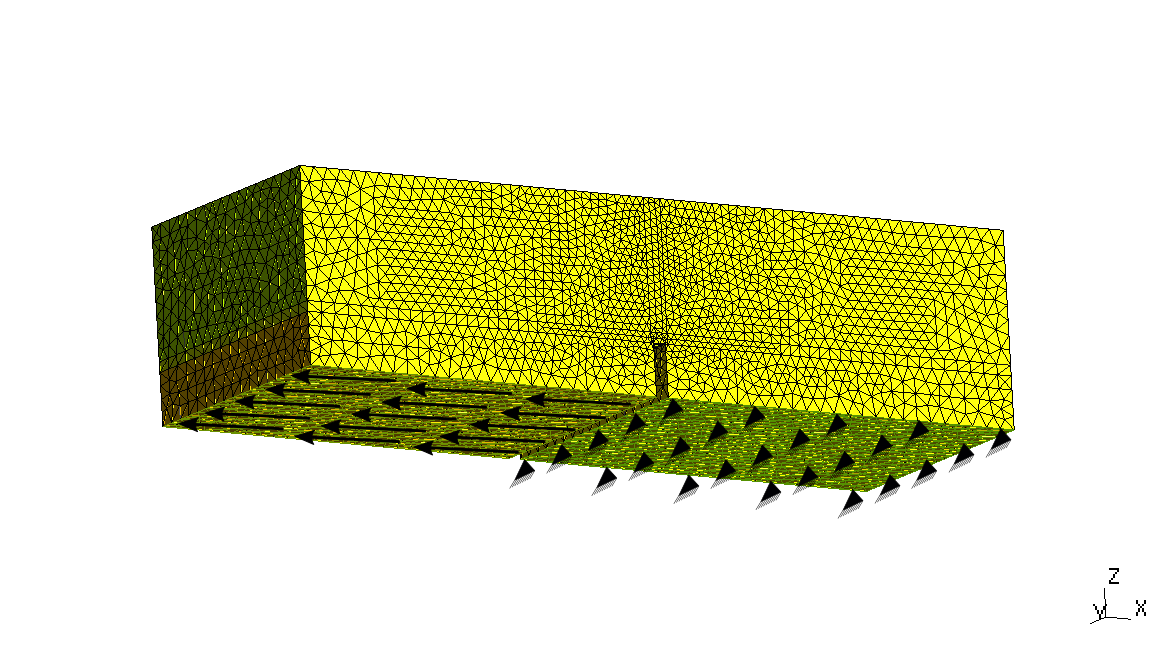
\includegraphics[width=0.4\textwidth]{img/modelo_condiciones}}
	\subfigure[crokis simplificado del modelo]{\label{fig:modelo_crokis} 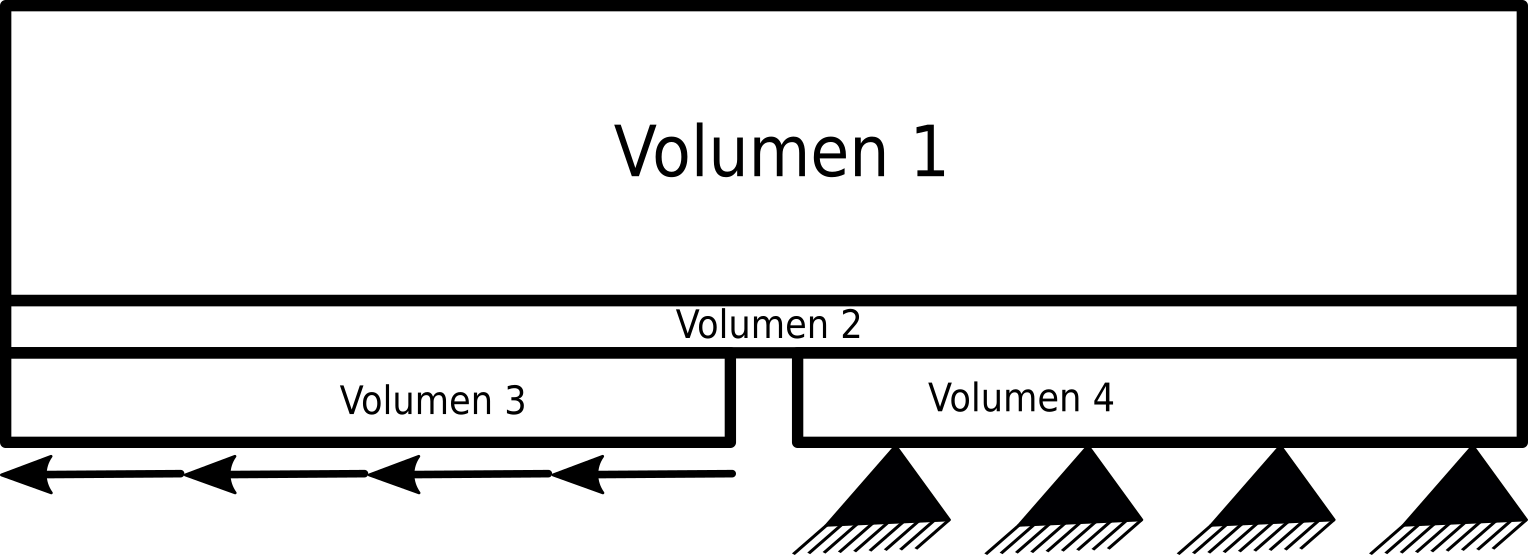
\includegraphics[width=0.4\textwidth]{img/modelo_crokis.png}}
	\caption{Modelo} \label{fig:modelo}
\end{figure}

Se ensallaran dos situaciones:

\begin{itemize}
	\item[Simualcion 1:] para la primera prueba, se ensaya un material homogéneo, es decir, todos los volúmenes del van a contener las mismas propiedades, imitando el ensayo original, donde era una probeta de hormigón solamente. 
	\item[Simualcion 2:] como segundo ensayo, y como propuesta nuestra, se realizara el modelo utilizando un material con distinta elasticidad como intercapa (Figura \ref{fig:modelo_crokis}: volumen 2), el cual podría ser un tipo de geo-textil, el cual buscara reducir las tensiones de tracción en el hormigón del volumen 1, de esta forma evitar la fisuración y aumentar su vida util.
	
	Se propone a este ultimo 2 alternativas, un material mas rígido y uno mas elástico
\end{itemize}

Por falta de mayor precision en la información, se utilizara valores medios, propuestos por los reglamentaciones vigentes

\section{Formulación variacional}
Las ecuaciones que gobiernan las deformaciones elásticas pequeñas de un cuerpo pueden ser escritas como se muestra en la expresión \ref{equ:defelas}:


\begin{subequations}
	\begin{equation}
		- \nabla \cdot \sigma  = f  \quad \quad \quad en \, \Omega
		\label{equ:defelas-a}
	\end{equation}
	\begin{equation}
		\sigma  = \lambda \cdot tr(\epsilon) \cdot I + 2 \cdot \mu \cdot \epsilon \quad \quad en \, \Omega
		\label{equ:defelas-b}
	\end{equation}
	\begin{equation}
		\epsilon  = \frac{1}{2} \cdot (\nabla u + (\nabla u)^t) \quad \quad en \, \Omega
		\label{equ:defelas-c}
	\end{equation}
	\label{equ:defelas}
\end{subequations}

Donde:
\begin{itemize}
	\item $\sigma$: es el tensor de tensiones
	\item $f$: es la fuerza de cuerpo por unidad de volumen.
	\item $\lambda y \mu]$: son los parámetros de elasticidad de Lamé del material en $\Omega$.
	\item $I$: es el tensor identidad.
	\item $tr$: es el operador traza de un tensor
	\item $\epsilon$: es el tensor de deformación unitaria simétrico (gradiente simétrico)
	\item $u$: es el campo vectorial de desplazamientos. 
\end{itemize}

Cuando hablamos de una integración en el tiempo, ya que este modelo es un ensayo elasto-dinámico, en lugar de usar la expresión \ref{equ:defelas-a}, se usa la \ref{equ:momenolineal}, donde se plantea el equilibrio del momento lineal.

\begin{equation}
	\nabla \cdot \sigma+ \rho b = \rho \ddot{u}
	\label{equ:momenolineal}
\end{equation}

En donde $u$ es el campo vectorial de desplazamiento, $\ddot{u}$ es la aceleración, $\rho$ la densidad del material, $b$ una fuerza en la masa.

Si combinamos \ref{equ:defelas-b} y \ref{equ:defelas-c}, se obtiene:

\begin{equation}
	\sigma = \lambda (\nabla \cdot u)I + \mu(\nabla u+(\nabla u)^t)
	\label{equ:momenolineal}
\end{equation}

Las ecuaciones \ref{equ:defelas} pueden ser fácilmente transformadas en un único vector de EPD para $u$, el cual es la PDE para el $u$ desconocido (Ecuación de Navier). Sin embargo, en la derivación de la formulación variacional, es conveniente mantener las ecuaciones separadas.

La forma débil se obtiene fácilmente integrando por partes la ecuación de equilibrio mediante una función de prueba $v \in V$ siendo $V$ un espacio de función adecuado que satisface las condiciones límite de desplazamiento:

\begin{equation}
	\int_{\Omega} \rho \ddot{u} \cdot v \,dx + \int_{\Omega} \sigma(u):\epsilon(v) \, dx = \int_{\Omega} \rho b \cdot v \, dx + \int_{\delta \Omega} (\sigma \cdot n) \cdot v \, ds \quad \quad \forall v \in V
	\label{equ:defelas-com}
\end{equation}

Se pueden introducir términos disipativos a nivel de la ecuación constitutiva si estos mecanismos son bien conocidos, pero con bastante frecuencia no es así. La disipación puede entonces modelarse añadiendo a la ecuación de evolución anterior un término de amortiguación en función de la velocidad $ \dot{u} $

Cuando se sabe poco sobre el origen de la amortiguación en la estructura, una elección popular para la matriz de amortiguación, conocida como amortiguación de Rayleigh, consiste en utilizar una combinación lineal de la matriz de masa y rigidez $[C]= \nu_M [M]+ \nu_K [K]$ con dos parámetros positivos $\nu_M$ $\nu_K$ que se pueden ajustar a las medidas experimentales.

\subsection{Discretización del Tiempo}

Ahora introducimos una discretizacion de tiempo del estudio del intervalo $[0;T]$ en incrementos de tiempo $N+1$ $t_0=0,t_1,...,t_N,t_{N+1}=T$ con $\Delta t=\frac{T}{N}$ que denota el paso de tiempo (supuesto constante). La resolución hará uso del método generalizado-$\alpha$ que puede ser visto como una extensión del ampliamente utilizado método de $Newmark-\beta$. Como método implícito, es incondicionalmente estable para una elección adecuada de los coeficientes, de modo que se pueden utilizar pasos de tiempo bastante grandes. También ofrece una precisión de segundo orden.

El método consiste en resolver la ecuación de evolución dinámica en un tiempo intermedio entre $t_N$ y $t_{N+1}$, de la siguiente manera

\begin{equation}
	[M](\ddot{u}_{n+1-\alpha_m})+[C](\dot{u}_{n+1-\alpha_f})+[K](u_{n+1-\alpha_m})=F(t_{n+1-\alpha_m})
\end{equation}

Con las siguientes aproximaciones:

\begin{equation}
	u_{n+1} = u_n + \Delta t(\dot{u}_n) + \frac{\Delta t^2}{2}((1-2\beta)\ddot{u}_n + 2 \beta \ddot{u}_{n+1})
	\dot{u}_{n+1} = \dot{u}_n + \Delta t((1- \gamma )\ddot{u}_n) + \gamma \ddot{u}_{n+1})
\end{equation}

\section{Procedimiento}

Todo el codigo del proyecto se encuentra subido a GitHub: \url{https://github.com/driendro/fatiga_asfalto_fem}

Se utilizo un scripts realizado con Python 3, en donde, con la librería \textbf{pygmsh} definimos la geometría de la pieza en 3D, a través de una función, lo que nos permite, variar fácilmente los parámetros de la geometría de la probeta. Luego, utilizando el mallado de GMSH, obtenemos un mallado de la superficie y el volumen. Por ultimo, luego de convertir la malla a xml usando \textbf{dolfin-convert}, con el fin de que "FEniCS" pueda interpretar los nodos y etiquetas de los diferentes volúmenes y superficies.

\subsubsection{Codigo}

El scripts de Python consta de 2 archivos, el primero esta definida la función que diseña la geometría, usando pygmsh, el segundo es el scripts, que desarrolla el calculo en si.

\paragraph{geometria.py} Este archivo se divide en las siguientes partes:

\begin{enumerate}
	\item Defecciones de la geometría de la probeta, tomadas de los parámetros de la función
	\item Puntos de que definen la geometría
	\item Lineas, bordes, superficies y volúmenes definidos.
	\item definimos los valores físicos del volumen y la superficie.
	\item creamos la malla y el xml, con la información para FEniCS. 
\end{enumerate}

Cabe aclarar que en la zona central, se dimensiona un sector al cual se le puede aumentar la densidad de puntos para un mejor detallado de la información.

\paragraph{calculo.py} Este archivo cuenta con la lógica del procesamiento de la simulación:

\begin{enumerate}
	\item Parámetros dimensionales de la geometría (tamaños y espesores)
	\item Compara para no regenerar la malla siempre.
	\item Clases que definen las propiedades de los materiales para cada parte de la probeta
	\item Parámetros de Elasticidad y coeficiente de Poisson.
	\item Clases que definen las funciones de calculo, y por ultimo el calculo por EF. 
\end{enumerate}


En el modelo geométrico, se definieron 4 volúmenes (Figura \ref{fig:vol}) y 2 superficies (bordes) (Figura \ref{fig:bord}), las cuales tendrán las condiciones de borde para la simulación.

\begin{figure}[h]
	\centering
	\subfigure[Volumenes]{\label{fig:vol} 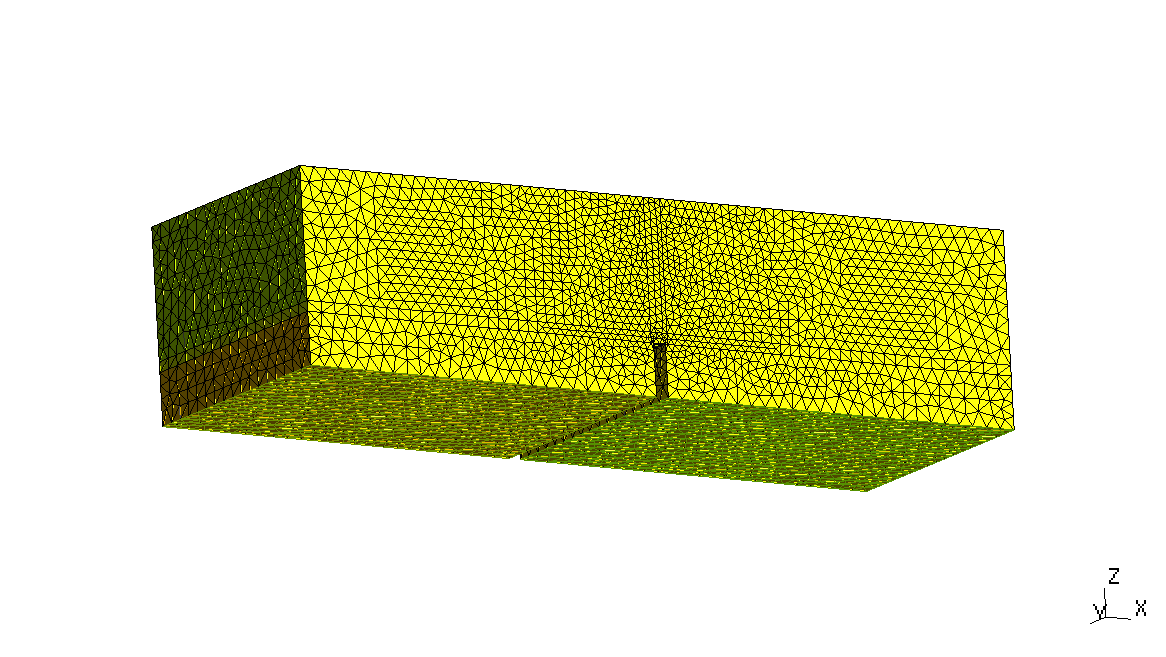
\includegraphics[width=0.4\textwidth]{img/modelo.png}}
	\subfigure[Bordes]{\label{fig:bord} 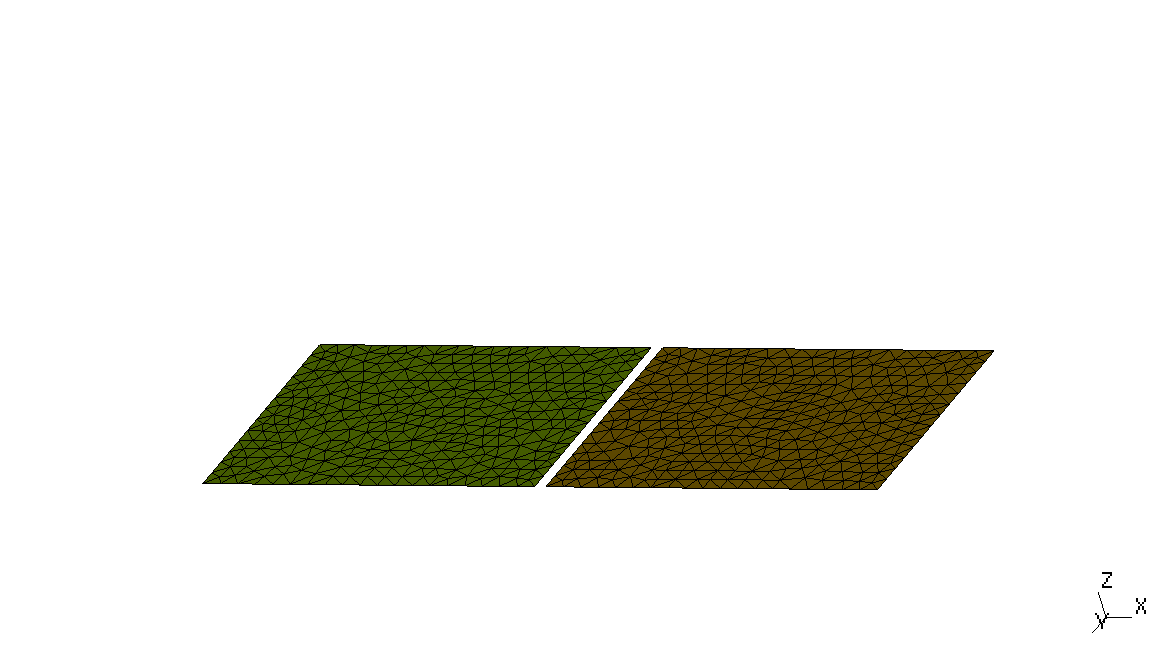
\includegraphics[width=0.4\textwidth]{img/modelo_sup.png}}
	\caption{Modelo} \label{fig:modelo1}
\end{figure}


\subsection{Simulaciónes}

Para todas las simulaciones las condiciones de borde se mantienen, todas las superficies del modelo se encuentran libres, salvo las mostradas en la figura \ref{fig:bord}, en este caso, el borde de la derecha se encuentra sujeto ($desplazamiento=0$), y el de la izquierda es cargado con una fuerza $P$ equivalente al $E$ ($P=E/20000$) del Hormigón (Expresión \ref{equ:fuerza_1}), hacia la derecha, separando las bases inferiores.

\begin{equation}
	\left\{\begin{matrix}
		p=p \cdot \frac{t}{tc} & 0<t<tc \\ 
		p=0 & tc<t<T
		\end{matrix}
		\right.
	\label{equ:fuerza_1}
\end{equation}

Donde:
\begin{itemize}
	\item T: Tiempo relativo del ensayo.
	\item tc: Tiempo de corte.
	\item pc: Valor de la fuerza máxima
\end{itemize}


\subsubsection{Simulacion 1}

Todo el material es Hormigón, con las siguientes propiedades

\begin{equation*}
	E=20000 MPa = 20000000 \frac{kn}{m^2} \\
	\nu = 0.2 \\
	\rho = 24 \frac{kn}{m^3}
\end{equation*}
 
\begin{figure}[h]
	\centering
	\subfigure[Tensiones]{\label{fig:sim1-sig} 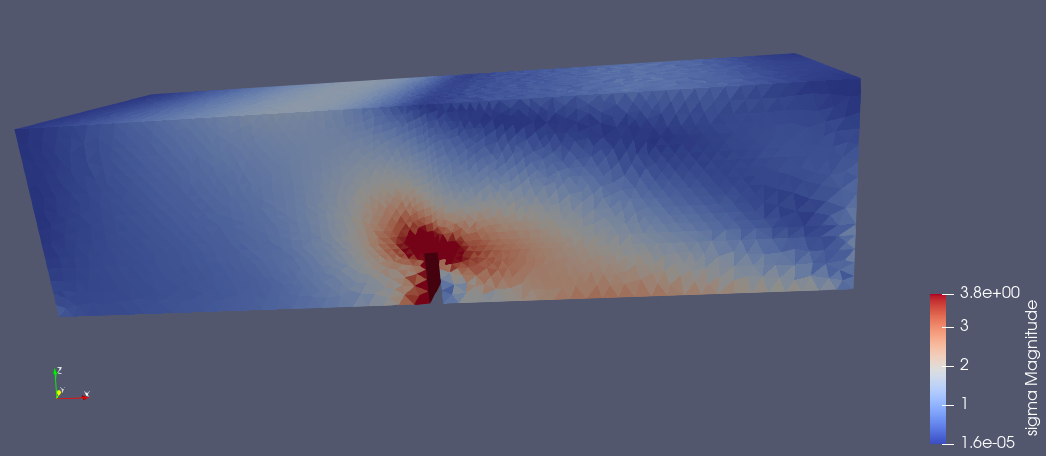
\includegraphics[width=0.45\textwidth]{img/1/sigma.png}}
	\subfigure[Tension y Deformacion]{\label{fig:sim1-def} 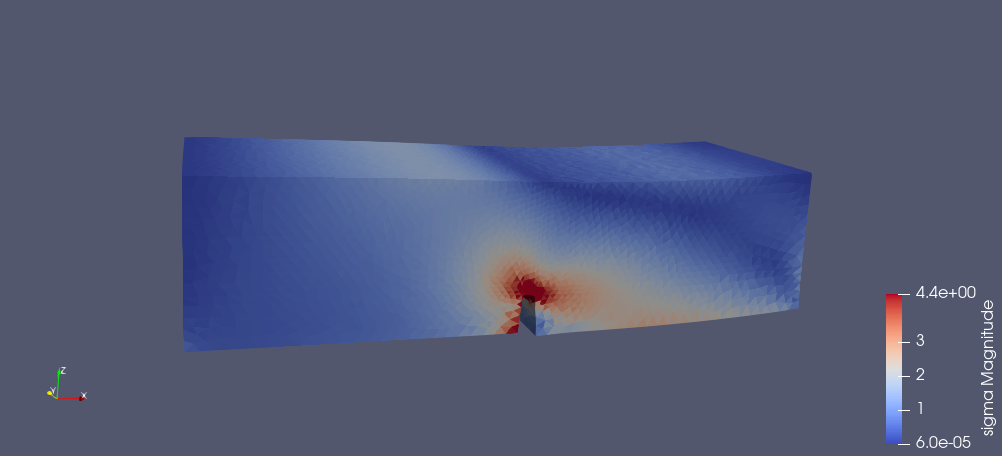
\includegraphics[width=0.45\textwidth]{img/1/def-sig}}
	\caption{Simulación 1: Todo Hormigón}
\end{figure}

\subsubsection{Simulacion 2-a}

Las propiedades de los volúmenes 1, 3 y 4, se mantienen a la de la simulación anterior, solo se pone en el volumen 2 un material mas rígido.

Para el los volúmenes 1,3 y 4
\begin{equation*}
	E=20000 MPa = 20000000 \frac{kn}{m^2} \\
	\nu = 0.2 \\
	\rho = 24 \frac{kn}{m^3}
\end{equation*}

Para el volumen 2
\begin{equation*}
	E=10000 MPa = 10000000 \frac{kn}{m^2} \\
	\nu = 0.2 \\
	\rho = 10 \frac{kn}{m^3}
\end{equation*}

\begin{figure}[h]
	\centering
	\subfigure[Tensiones]{\label{fig:sim2-sig} 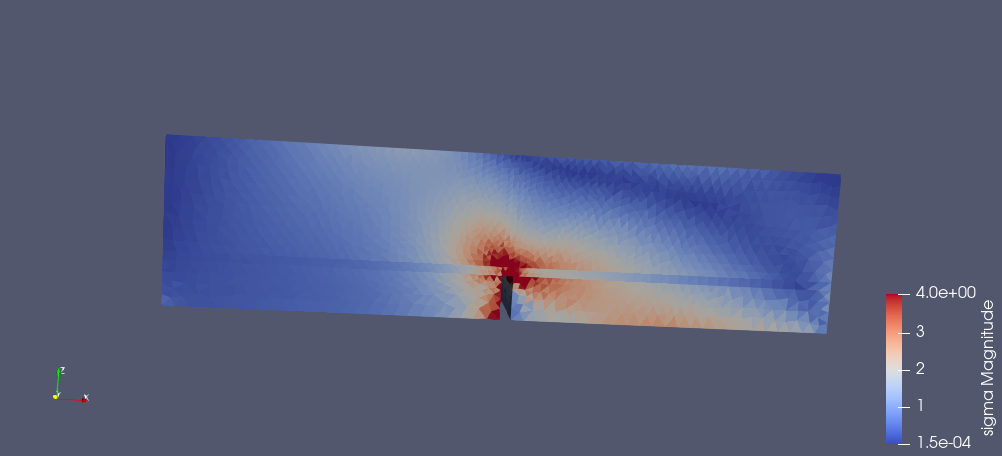
\includegraphics[width=0.45\textwidth]{img/2/sigma.png}}
	\subfigure[Tension y Deformacion]{\label{fig:sim2-def} 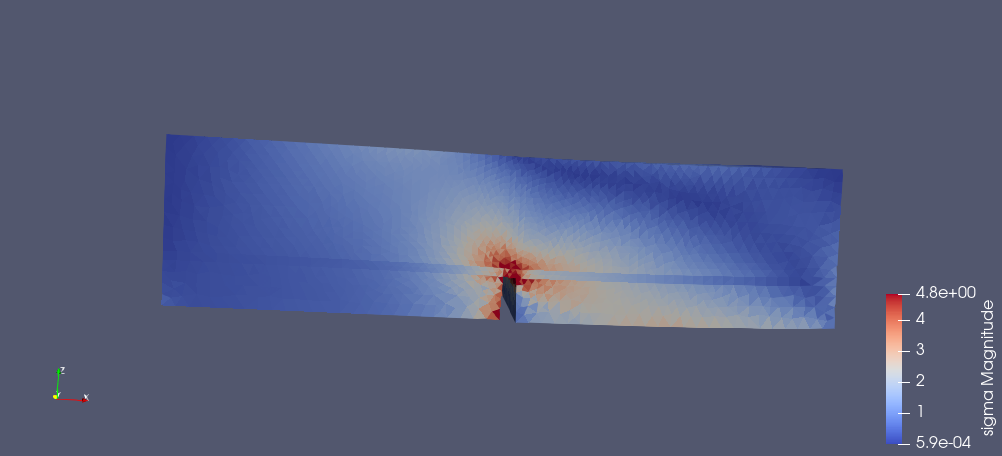
\includegraphics[width=0.45\textwidth]{img/2/def-sig}}
	\caption{Simulación 2-a: Intercapa rígida}
\end{figure}

\subsection{Simulación 2-b}

Las propiedades de los volúmenes 1, 3 y 4, se mantienen a la de la simulación anterior, solo se pone en el volumen 2 un material mas elástico.

Para el los volúmenes 1,3 y 4
\begin{equation*}
	E=20000 MPa = 20000000 \frac{kn}{m^2} \\
	\nu = 0.2 \\
	\rho = 24 \frac{kn}{m^3}
\end{equation*}

Para el volumen 2
\begin{equation*}
	E=40000 MPa = 40000000 \frac{kn}{m^2} \\
	\nu = 0.2 \\
	\rho = 10 \frac{kn}{m^3}
\end{equation*}

\begin{figure}[h]
	\centering
	\subfigure[Tensiones]{\label{fig:sim3-sig} 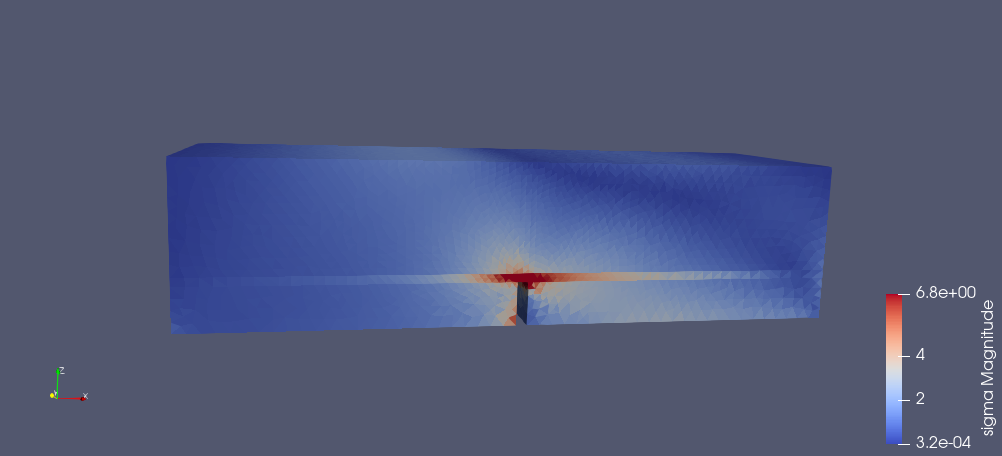
\includegraphics[width=0.45\textwidth]{img/3/sigma.png}}
	\subfigure[Tension y Deformacion]{\label{fig:sim3-def} 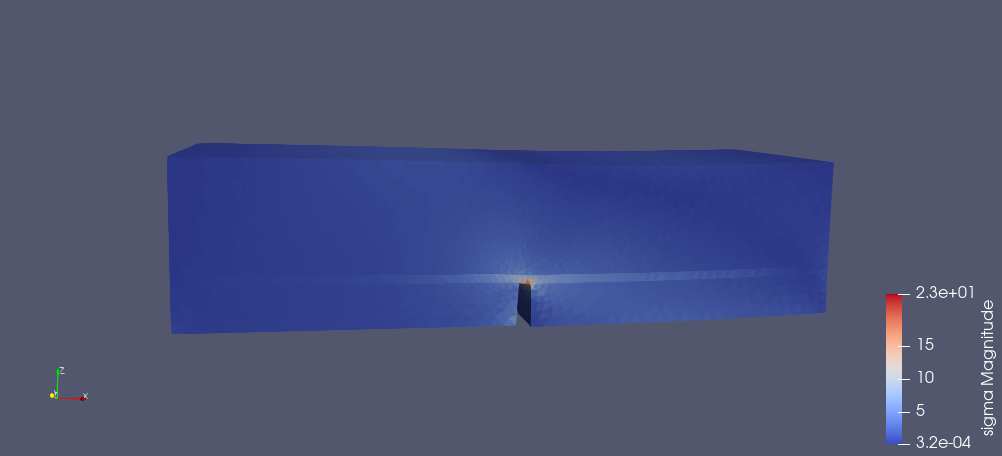
\includegraphics[width=0.45\textwidth]{img/3/def-sig}}
	\caption{Simulación 2-b: Intercapa elástica}
\end{figure}

\subsection{Conclusiones}


Comparando los resultados arrojados por las simulaciones, en los tres casos, existe una elevada concentración de tensiones en el área central, sobre todo cerca de la ranura.

Un resumen se muestra en la Tabla \ref{tab:resumen}.

\begin{table}[h]
	\resizebox{0.5\textwidth}{!}{%
	\begin{tabular}{|c|c|c|}
	\hline
	Simulación & Sigma & Deformación \\ \hline
	1 & 1,5 & 3,4 \\ \hline
	2 & 9,7 & 3,6 \\ \hline
	3 & 17 & 3,5 \\ \hline
	\end{tabular}%
	}
	\caption[Resumen]{Valores de la tensión y la deformación en cada simulación}
	\label{tab:resumen}
\end{table}

Al intercalar un material con distinta elasticidad se observan mejoras en el comportamiento, desarrollándose menores valore de tensión, en el hormigón, ya que la absorbe el material interno entre las capas.

\end{document}
